\section{Operationsverstaerker}

\subsection{Eigenschaften eines OpAmps}

\begin{minipage}{0.6\columnwidth}
	\begin{center}
		% LTeX: enabled=false
\resizebox{0.6\columnwidth}{!}{
    \begin{circuitikz}
        \tikzstyle{every node}=[font=\Huge]
        \draw [line width=1pt, short] (0,0) -- (7.75,4.5);
        \draw [line width=1pt, short] (0,0) -- (0,9);
        \draw (4.25,4.5) to[american voltage source] (2.75,3);
        \draw [line width=1pt, short] (7.75,4.5) -- (0,9);
        \node at (1,2.5) {\textbf{+}};
        \node at (1,6.5) {\textbf{-}};
        \draw (0.5,2.5) to[european resistor] (0.5,6.5);
        \draw (0.5,2.5) to[short, -o] (-1.75,2.5) ;
        \draw (0.5,6.5) to[short, -o] (-1.75,6.5) ;
        \draw [<->, >=Stealth] (-0.5,2.5) -- (-0.5,6.5)node[pos=0.5, fill=white]{$V_{in}$};
        \node at (1.75,4.5) {$Z_i = \infty$};
        \draw (2.75,3) to (2.75,2.75) node[ground]{};
        \node at (4.5,3.25) {$a = \infty$};
        \draw (4.25,4.5) to[european resistor] (6,4.5);
        \draw (6,4.5) to[short, -o] (9,4.5) ;
        \draw [->, >=Stealth] (-2,2) -- (-0.25,2)node[pos=0.5, fill=white]{$I_{in}=0$};
        \node at (8.5,5) {$V_{out}$};
        \draw [->, >=Stealth] (-1.75,7) -- (-0.25,7)node[pos=0.5, fill=white]{$I_{in}=0$};
        \node at (5,5) {$Z_{out} = 0$};
    \end{circuitikz}
}%
%Tikzmaker code:
%[[],[{"x":0,"y":850},{"x":387.5,"y":625},"Line",1,"\\draw [line width=1pt, short] (0,0) -- (7.75,4.5);","",[0,0,0],[255,255,255],0,false,[0,0,0,0],1,{"fontSize":32,"textPlacement":0.5,"isBold":false,"isItalic":false,"hasUnderline":false,"alignmentText":"center"}],[{"x":0,"y":850},{"x":0,"y":400},"Line",3,"\\draw [line width=1pt, short] (0,0) -- (0,9);","",[0,0,0],[255,255,255],0,false,[0,0,0,0],1,{"fontSize":32,"textPlacement":0.5,"isBold":false,"isItalic":false,"hasUnderline":false,"alignmentText":"center"}],[{"x":212.5,"y":625},{"x":137.5,"y":700},"Voltage Source (American)",5,"\\draw (4.25,4.5) to[american voltage source] (2.75,3);","",[0,0,0],[255,255,255],0,false,32,0.4,{"isBold":false,"isItalic":false,"hasUnderline":false,"rotation":0,"frequency":1,"amplitude":1,"phase":0,"multiwire":0,"alignmentText":"center","endNodeType":"circ"}],[{"x":387.5,"y":625},{"x":0,"y":400},"Line",7,"\\draw [line width=1pt, short] (7.75,4.5) -- (0,9);","",[0,0,0],[255,255,255],0,false,[0,0,0,0],1,{"fontSize":32,"textPlacement":0.5,"isBold":false,"isItalic":false,"hasUnderline":false,"alignmentText":"center"}],[{"x":50,"y":725},{"x":50,"y":725},"Text",8,"\\node [font=\\LARGE] at (1,2.5) {\\textbf{+}};","+",[0,0,0],[255,255,255],0,false,32,0.4,{"isBold":true,"isItalic":false,"hasUnderline":false,"rotation":0,"frequency":1,"amplitude":1,"phase":0,"multiwire":0,"alignmentText":"center","endNodeType":"circ","isMathMode":false}],[{"x":50,"y":525},{"x":50,"y":525},"Text",9,"\\node [font=\\LARGE] at (1,6.5) {\\textbf{-}};","-",[0,0,0],[255,255,255],0,false,32,0.4,{"isBold":true,"isItalic":false,"hasUnderline":false,"rotation":0,"frequency":1,"amplitude":1,"phase":0,"multiwire":0,"alignmentText":"center","endNodeType":"circ","isMathMode":false}],[{"x":25,"y":725},{"x":25,"y":525},"Resistor (IEC)",10,"\\draw (0.5,2.5) to[european resistor] (0.5,6.5);","",[0,0,0],[255,255,255],0,false,32,0.4,{"isBold":false,"isItalic":false,"hasUnderline":false,"rotation":0,"frequency":1,"amplitude":1,"phase":0,"multiwire":0,"alignmentText":"center","endNodeType":"circ","isMathMode":true}],[{"x":25,"y":725},{"x":-87.5,"y":725},"End node",12,"\\draw [](0.5,2.5) to[short, -o] (-1.75,2.5) ;","",[0,0,0],[255,255,255],0,false,32,0.4,{"isBold":false,"isItalic":false,"hasUnderline":false,"rotation":0,"frequency":1,"amplitude":1,"phase":0,"multiwire":0,"alignmentText":"center","endNodeType":"circ"}],[{"x":25,"y":525},{"x":-87.5,"y":525},"End node",13,"\\draw [](0.5,6.5) to[short, -o] (-1.75,6.5) ;","",[0,0,0],[255,255,255],0,false,32,0.4,{"isBold":false,"isItalic":false,"hasUnderline":false,"rotation":0,"frequency":1,"amplitude":1,"phase":0,"multiwire":0,"alignmentText":"center","endNodeType":"circ"}],[{"x":-25,"y":725},{"x":-25,"y":525},"Double-headed arrow",14,"\\draw [<->, >=Stealth] (-0.5,2.5) -- (-0.5,6.5)node[pos=0.5,undefined, fill=white]{$V_{in}$};","V_{in}",[0,0,0],[255,255,255],0,false,[0,0,0,0],0.4,{"fontSize":32,"textPlacement":0.5,"isBold":false,"isItalic":false,"hasUnderline":false,"isMathMode":true}],[{"x":87.5,"y":625},{"x":87.5,"y":625},"Text",15,"\\node [font=\\Large] at (1.75,4.5) {$Z_i = \\infty$};","Z_i = \\infty",[0,0,0],[255,255,255],0,true,27,0.4,{"isBold":false,"isItalic":false,"hasUnderline":false,"isMathMode":true,"rotation":0}],[{"x":137.5,"y":700},{"x":137.5,"y":712.5},"Ground",16,"\\draw (2.75,3) to (2.75,2.75) node[ground]{};","",[0,0,0],[255,255,255],0,false,22,0.4,{"isBold":false,"isItalic":false,"hasUnderline":false,"isMathMode":true,"rotation":0,"frequency":1,"amplitude":1,"phase":0,"multiwire":0,"endNodeType":"circ"}],[{"x":212.5,"y":687.5},{"x":212.5,"y":687.5},"Text",19,"\\node [font=\\Large] at (4.25,3.25) {$a = \\infty$};","a = \\infty",[0,0,0],[255,255,255],0,false,27,0.4,{"isBold":false,"isItalic":false,"hasUnderline":false,"isMathMode":true,"rotation":0}],[{"x":212.5,"y":625},{"x":300,"y":625},"Resistor (IEC)",20,"\\draw (4.25,4.5) to[european resistor] (6,4.5);","",[0,0,0],[255,255,255],0,false,22,0.4,{"isBold":false,"isItalic":false,"hasUnderline":false,"isMathMode":true,"rotation":0,"frequency":1,"amplitude":1,"phase":0,"multiwire":0,"endNodeType":"circ"}],[{"x":300,"y":625},{"x":450,"y":625},"End node",23,"\\draw [](6,4.5) to[short, -o] (9,4.5) ;","",[0,0,0],[255,255,255],0,false,22,0.4,{"isBold":false,"isItalic":false,"hasUnderline":false,"isMathMode":true,"rotation":0,"frequency":1,"amplitude":1,"phase":0,"multiwire":0,"endNodeType":"circ"}],[{"x":-100,"y":750},{"x":-12.5,"y":750},"Arrow",24,"\\draw [->, >=Stealth] (-2,2) -- (-0.25,2)node[pos=0.5,undefined, fill=white]{$I_{in}=0$};","I_{in}=0",[0,0,0],[255,255,255],0,false,[0,0,0,0],0.4,{"fontSize":22,"textPlacement":0.5,"isBold":false,"isItalic":false,"hasUnderline":false,"isMathMode":true}],[{"x":425,"y":600},{"x":425,"y":600},"Text",26,"\\node [font=\\Large] at (8.5,5) {$V_{out}$};","V_{out}",[0,0,0],[255,255,255],0,false,27,0.4,{"isBold":false,"isItalic":false,"hasUnderline":false,"isMathMode":true,"rotation":0}],[{"x":-87.5,"y":500},{"x":-12.5,"y":500},"Arrow",27,"\\draw [->, >=Stealth] (-1.75,7) -- (-0.25,7)node[pos=0.5,undefined, fill=white]{$I_{in}=0$};","I_{in}=0",[0,0,0],[255,255,255],0,false,[0,0,0,0],0.4,{"fontSize":27,"textPlacement":0.5,"isBold":false,"isItalic":false,"hasUnderline":false,"isMathMode":true}],[{"x":250,"y":600},{"x":250,"y":600},"Text",28,"\\node [font=\\Large] at (5,5) {$Z_{out} = 0$};","Z_{out} = 0",[0,0,0],[255,255,255],0,false,27,0.4,{"isBold":false,"isItalic":false,"hasUnderline":false,"isMathMode":true,"rotation":0}]]
		% 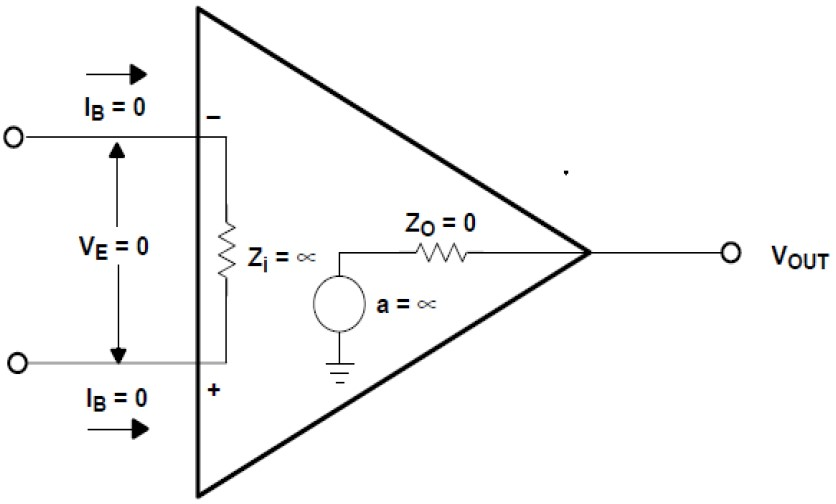
\includegraphics[width=0.7\columnwidth]{images/OPV_1.jpg} 		
	\end{center}
\end{minipage}
\hfill
\begin{minipage}{0.38\columnwidth}
	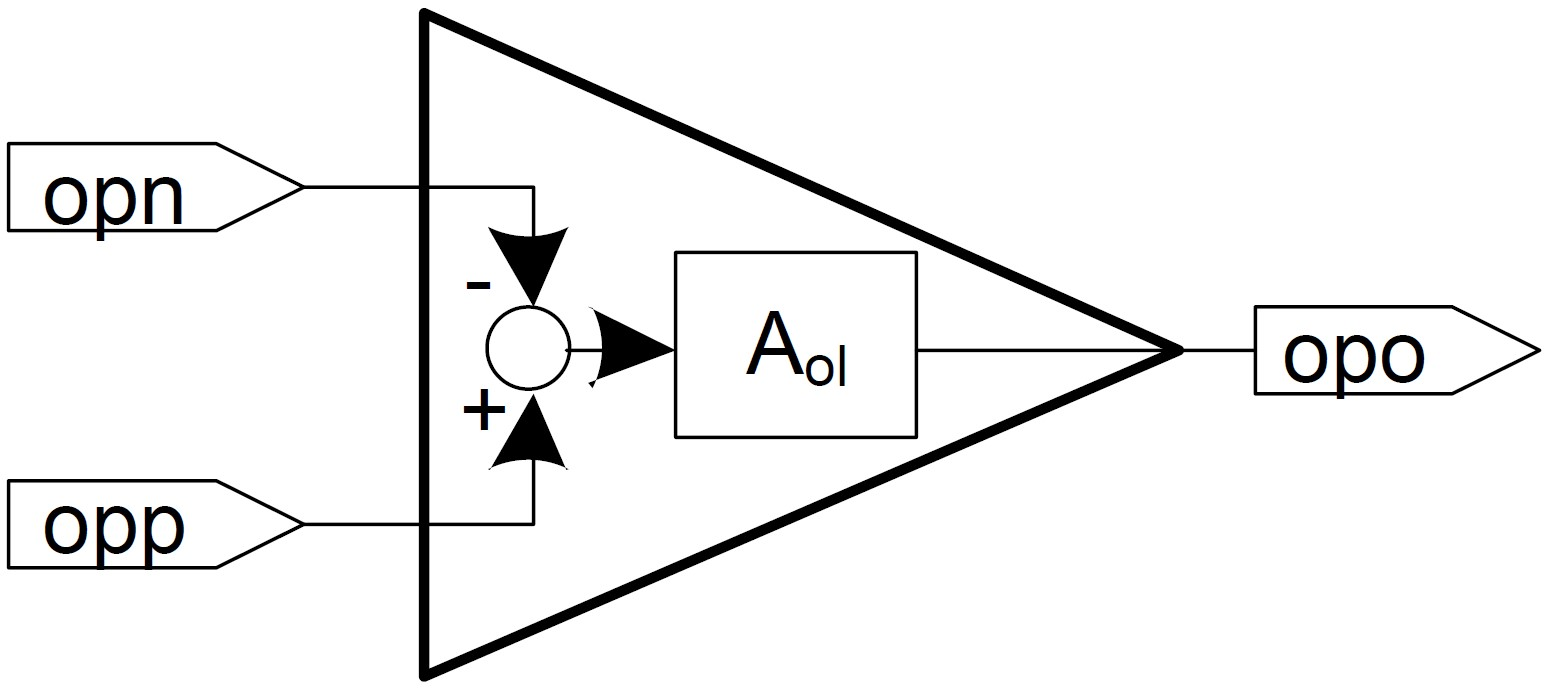
\includegraphics[width=0.8\columnwidth]{images/OPV_2.jpg} 
\end{minipage}


\subsection{OpAmp als Verstärker}

\begin{itemize}
	\item \textbf{Rückkopplung auf negativen Eingang}
	\item OpAmp stellt $V_{\rm out}$ so ein, dass beide Eingänge die gleiche Spannung aufweisen\\
		\textrightarrow\ $V_{\rm opn} = V_{\rm opp}$
	\item \textbf{opn ist virtueller Massepunkt}
	\item Lineare Schaltung (solange nicht am Anschlag) \textrightarrow\ Superposition
	\item \cbl{für $A_{\rm ol} \neq \infty$} $V_{\rm opn}$ als Spannungsteiler von $V_{\rm out}$ zu ausgeschaltetem $V_{in_i}$ durch \\
		Superposition  ausdrücken
\end{itemize}


\begin{minipage}[c]{0.48\columnwidth}
	$$ V_{\rm out} = A_{\rm ol} \cdot (V_{\rm opp} - V_{\rm opn}) $$
\end{minipage}
\hfill
\begin{minipage}[c]{0.48\columnwidth}
	$$ V_{\rm out} = A_{\rm ol} \cdot (V_{\rm in} + V_{\rm os} - V_{\rm opn} ) $$ 
\end{minipage}


\subsection{Grundschaltungen OpAmp}

\subsubsection{Nicht-Invertierender Verstärker}

\begin{minipage}[c]{0.4\columnwidth}
	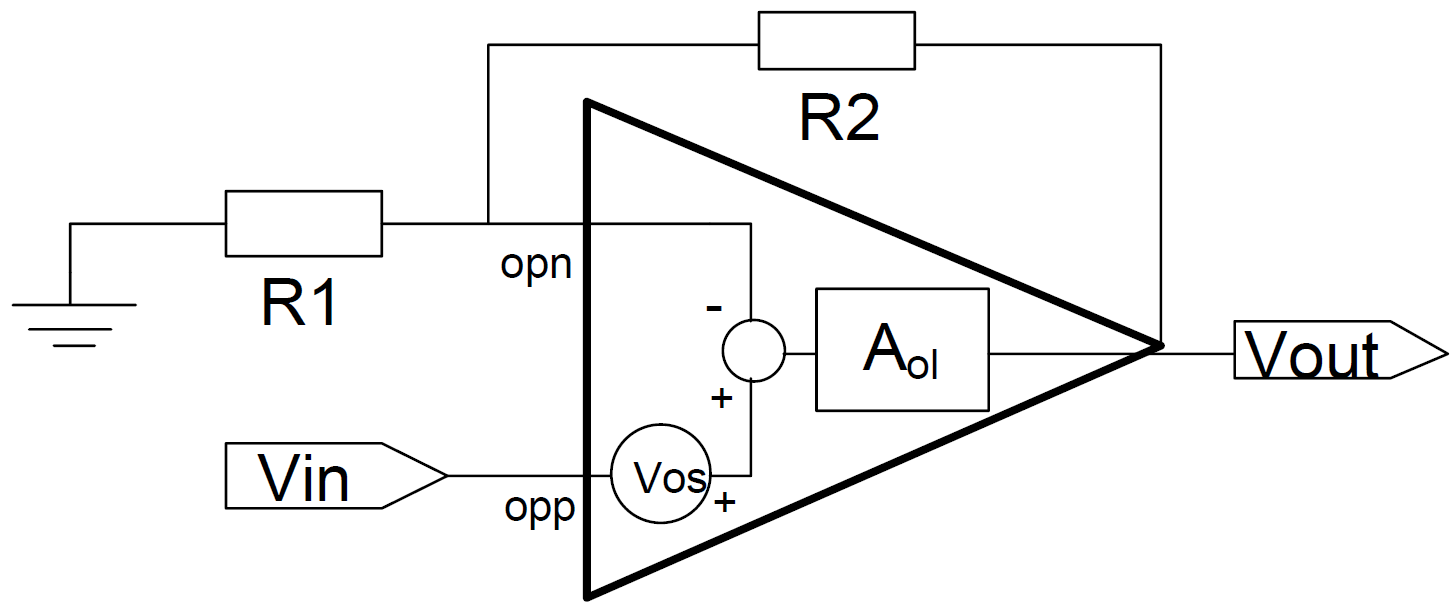
\includegraphics[width=\columnwidth]{images/nicht-invertierender_verstaerker_offset.png}
\end{minipage}
\hfill
\begin{minipage}[c]{0.58\columnwidth}
	$$ V_{\rm opn} = (V_{\rm GND} + V_{\rm os}) \cdot \frac{R_2}{R_1 + R_2} + \frac{R_1}{R_1 + R_2} \cdot V_{\rm out} $$ 
\end{minipage}


\begin{minipage}[t]{0.48\columnwidth}
	\textbf{Real}

	\vspace{0.1cm}

	\scalebox{0.8}{
	$ \boxed {\quad  V_{\rm out} = \frac{A_{\rm ol}}{1 + A_{\rm ol} \cdot \frac{R_1}{R_1 + R_2}} \cdot (V_{\rm in} + V_{\rm os}) - \frac{R_2}{R_1} \cdot A_{\rm GND} } $}
\end{minipage}
\hfill
\begin{minipage}[t]{0.5\columnwidth}
	\textbf{Ideal}

	\vspace{0.1cm}

	\scalebox{0.9}{
	$ \boxed { \quad V_{\rm out} = ( V_{\rm in} + V_{\rm os}) \cdot \frac{R_1 + R_2}{R_1} - \frac{R_2}{R_1} \cdot A_{\rm GND} } $}
\end{minipage}


\subsubsection{Invertierender Verstärker}

\begin{minipage}[c]{0.4\columnwidth}
	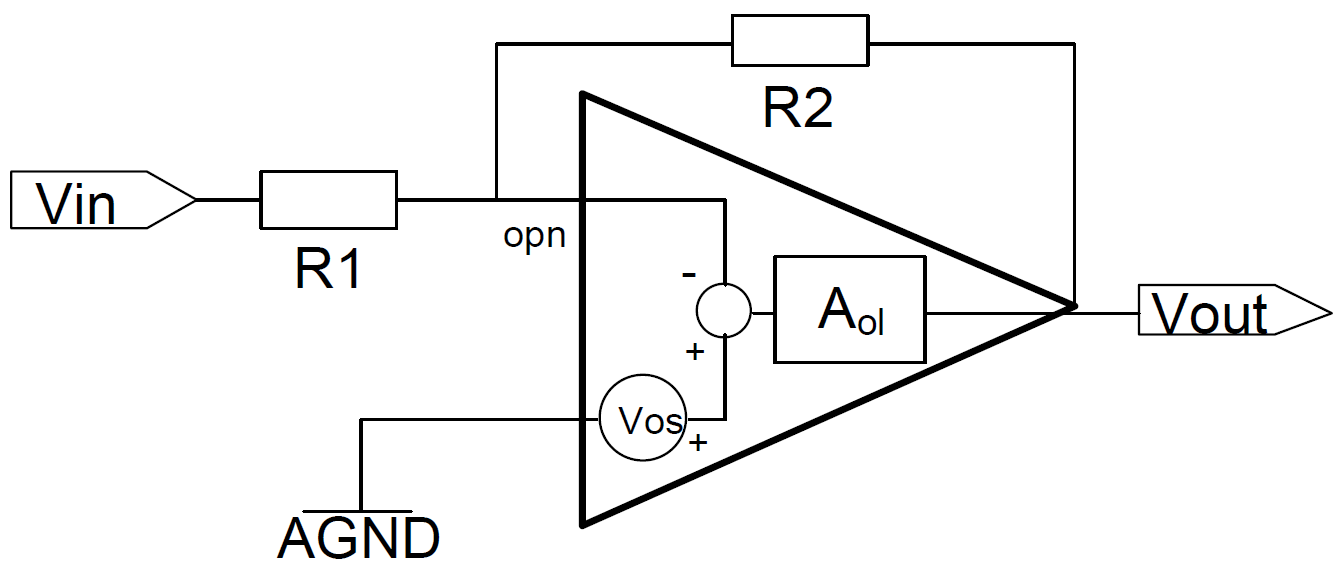
\includegraphics[width=0.9\columnwidth]{images/invertierender_verstaerker_offset.png}
\end{minipage}
\hfill
\begin{minipage}[c]{0.58\columnwidth}
	Knoten: $I_2 - I_1 - I_{\rm opn} = 0$ mit $I_{\rm opn} = 0$: \quad  $I_2 = I_1$ 
	$$ I_1 = - \frac{V_{\rm in}}{R_1} \qquad V_{\rm out} = V_{R_2} = I_2 \cdot R_2 = I_1 \cdot R_2 $$
	$$ \boxed{ V_{\rm opn} = V_{\rm in} \cdot \frac{R_2}{R_1 + R_2} + V_{\rm out} \frac{R_1}{R_1 + R_2}} $$
\end{minipage}

\vspace{0.2cm}

\begin{minipage}[t]{0.54\columnwidth}
	\textbf{Real}

	\vspace{0.1cm}

	\scalebox{0.8}{
	% $ \boxed{ V_{\rm out} = \frac{A_{\rm ol}}{1+A_{\rm ol} \cdot \frac{R_1}{R_1 + R_2}} \cdot \Big( A_{\rm GND} + V_{\rm os} \Big) - V_{\rm in} \cdot \frac{R_2}{R_1}  } $
	$ \boxed{ V_{\rm out} = \frac{(R_1 + R_2) \cdot A_{\rm ol} \cdot (V_{\rm pos} + V_{\rm os}) - R_2 \cdot A_{\rm ol} \cdot V_{\rm neg} }{R_1 + R_2 +  R_1 \cdot A_{\rm ol}} }$
	}
\end{minipage}
\hfill
\begin{minipage}[t]{0.44\columnwidth}
	\textbf{Ideal}

	\vspace{0.1cm}

	\scalebox{0.8}{
	$ \boxed{ V_{\rm out} = \frac{R_1 + R_2}{R_1} \cdot \Big(  A_{\rm GND} + V_{\rm os} \Big) - V_{\rm in} \cdot \frac{R_2}{R_1} } $ }
\end{minipage}


\subsubsection{Invertierender Summierender Verstärker (Addierer)}

\begin{minipage}[c]{0.38\columnwidth}
	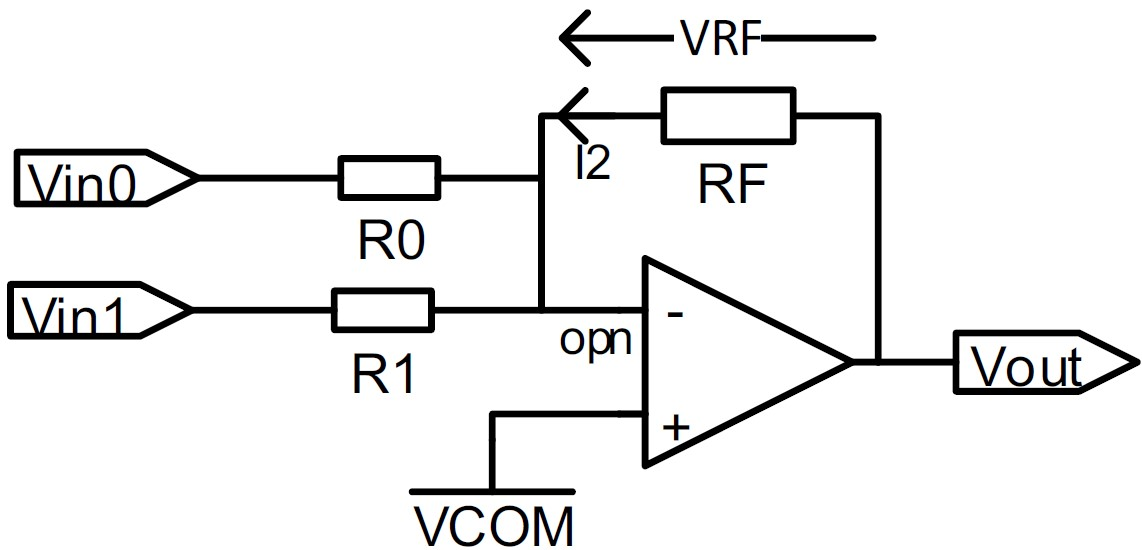
\includegraphics[width=\columnwidth]{images/invertierender_summierender_verstaerker.jpg}
\end{minipage}
\hfill
\begin{minipage}[c]{0.58\columnwidth}
	$$ I_2 - I_1 - I_0 = 0 \text{ \textrightarrow\ } I_2 = -I_1 - I_0 $$
	$$ I_0 = \frac{V_{\rm in0} - V_{\rm COM} - V_{\rm os}}{R_0} \quad I_1 = \frac{V_{in1} - V_{COM}- V_{\rm os}}{R_1} $$
\end{minipage}

\vspace{0.2cm}

$$ \boxed{ V_{\rm out} = (V_{\rm COM} + V_{\rm os}) \cdot \Bigg( \frac{R_f + R_0 || R_1}{R_0 || R_1} \Bigg)  - R_F \cdot \Bigg( \frac{V_{\rm in0}}{R_0} + \frac{V_{\rm in1}}{R_1} \Bigg) } $$


\subsubsection{Buffer}

\begin{minipage}[c]{0.48\columnwidth}
	\begin{center}
		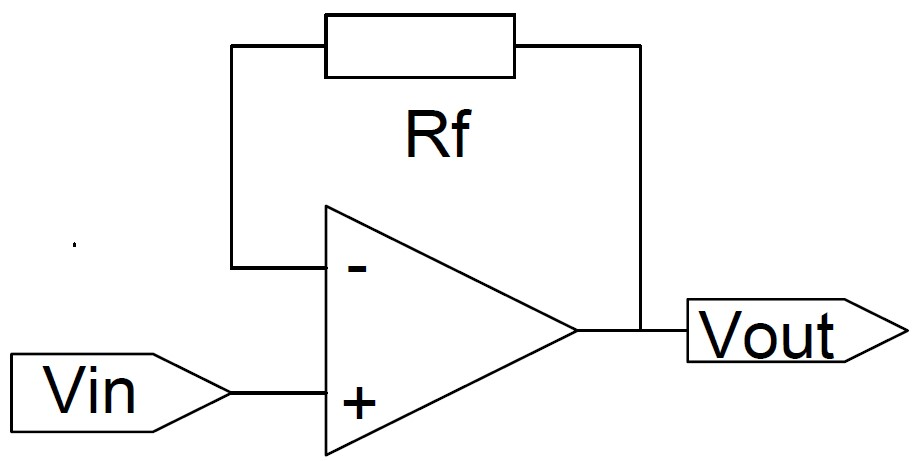
\includegraphics[width=0.65\columnwidth]{images/buffer_1.jpg}

		\begin{itemize}
			\item $V_{\rm out} = V_{\rm in} + V_{\rm os}$
			\item Keine Belastung an $V_{\rm in}$
		\end{itemize}
	\end{center}
\end{minipage}
\hfill
\begin{minipage}[c]{0.48\columnwidth}
	\begin{center}
		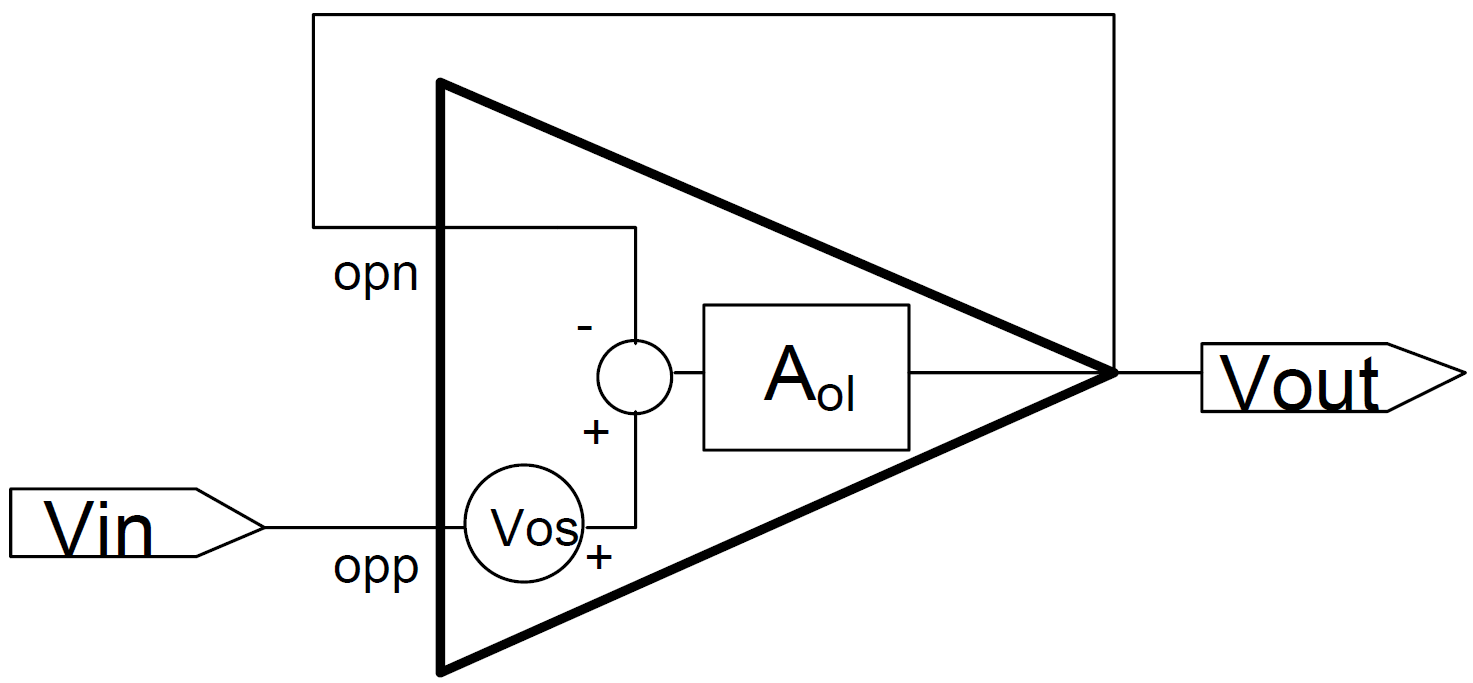
\includegraphics[width=0.7\columnwidth]{images/buffer_offset.png}

		\begin{itemize}
			\item Kopplungsfaktoren $= 1$
			\item Tiefer Ausgangswiderstand
		\end{itemize}
	\end{center}
\end{minipage}


\subsection{Analoge Rechenschaltungen mit OpAmps}

\subsubsection{Differenzverstärker (Gewichteter Subtrahierer)}

\begin{minipage}[c]{0.4\columnwidth}
	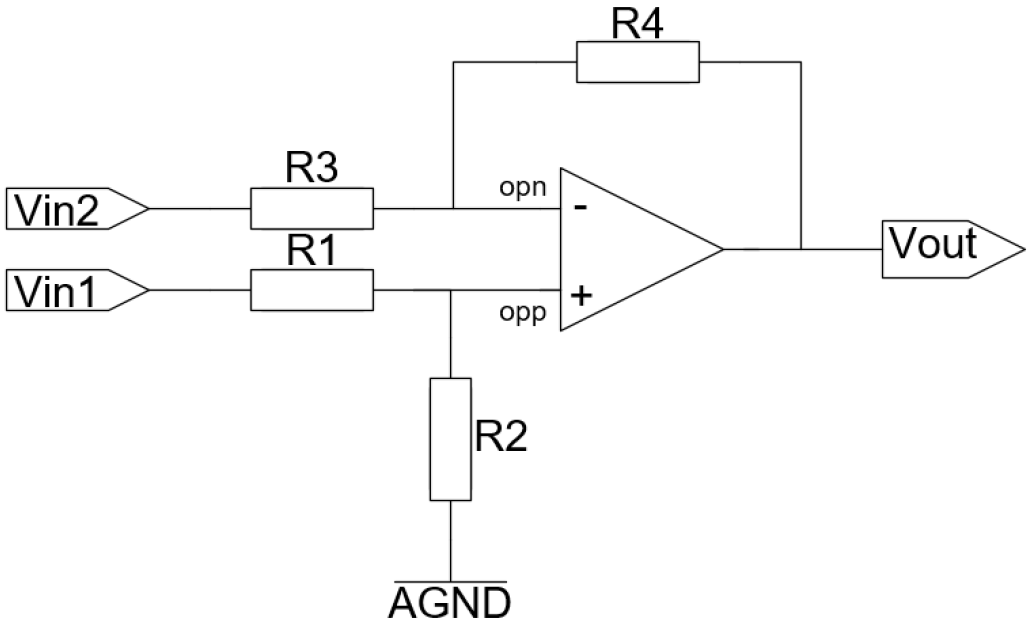
\includegraphics[width=\columnwidth]{images/differenzverstärker.png}
\end{minipage}
\hfill
\begin{minipage}[c]{0.58\columnwidth}
	\begin{tabular}{ll}
		oben:	& invertierender Verstärker			\\
		unten: 	& nicht-invertierender Verstärker 	\\
				& mit Spannungsteiler
	\end{tabular}
\end{minipage}

$$ \boxed{  V_{\rm out} = \frac{R_3 + R_4}{R_3} \cdot \Bigg( \frac{R_1}{R_1 + R_2} \cdot A_{\rm GND} + \frac{R_2}{R_1 + R_2} \cdot V_{\rm in1} \Bigg) - \frac{R_4}{R_3} \cdot V_{\rm in2} } $$
$$ \boxed{ \text{Für } R_1 = R_3, \, R_2 = R_4: \quad  V_{\rm out} =  A_{\rm GND} + \frac{R_4}{R_3} \cdot ( V_{\rm in1} - V_{\rm in2}) } $$


\subsubsection{Instrumentenverstärker}

OP1 und OP2 sind nicht-invertierende Verstärker mit gemeinsamem Widerstand $R_g$

\begin{minipage}[c]{0.5\columnwidth}
	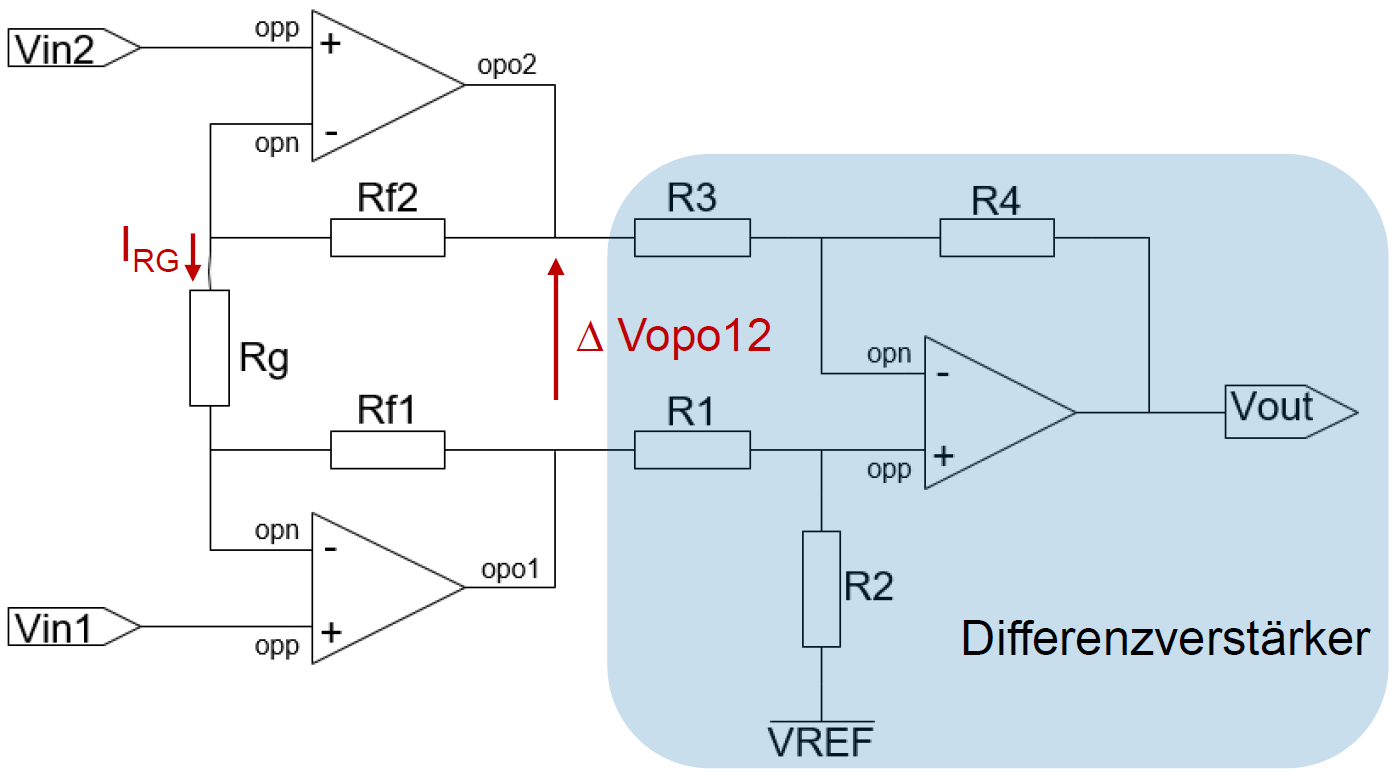
\includegraphics[width=\columnwidth]{images/instrumentenverstaerker.png}
\end{minipage}
\hfill
\begin{minipage}[c]{0.48\columnwidth}
	$$ I_{\rm Rg} = \frac{V_{\rm in2} - V_{\rm in1}}{R_g} $$
	$$ V_{\rm opo2} = V_{\rm in2} + \frac{R_{f2}}{R_g} \cdot(V_{\rm in2} - V_{\rm in1}) $$
	$$ V_{\rm opo1} = V_{\rm in1} + \frac{R_{f1}}{R_g} \cdot(V_{\rm in1} - V_{\rm in2}) $$
\end{minipage}

$$ \boxed{ \Delta V_{\rm opo12} = V_{\rm opo2} - V_{\rm opo1} = \Bigg( 1 + \frac{R_{f1} + R_{f2}}{R_g} \Bigg) \cdot(V_{\rm in1} - V_{\rm in2}) } $$
$$ \boxed{ \text{Für } R_1 = R_3, \, R_2 = R_4: \quad  V_{\rm out} =  V_{\rm REF} + \frac{R_4}{R_3} \cdot \Bigg( 1 + \frac{R_{f1} + R_{f2}}{R_g} \Bigg) \cdot(V_{\rm in1} - V_{\rm in2}) } $$


\columnbreak


\subsection{Mehrstufige Verstärker}

Für $\mathrm{AGND} \neq 0 \, \volt$ muss Superposition angewendet werden. \\
\textrightarrow\ $\mathrm{AGND}$ als Quelle annehmen und anderen Eingang 'ausschalten'

\begin{center}
	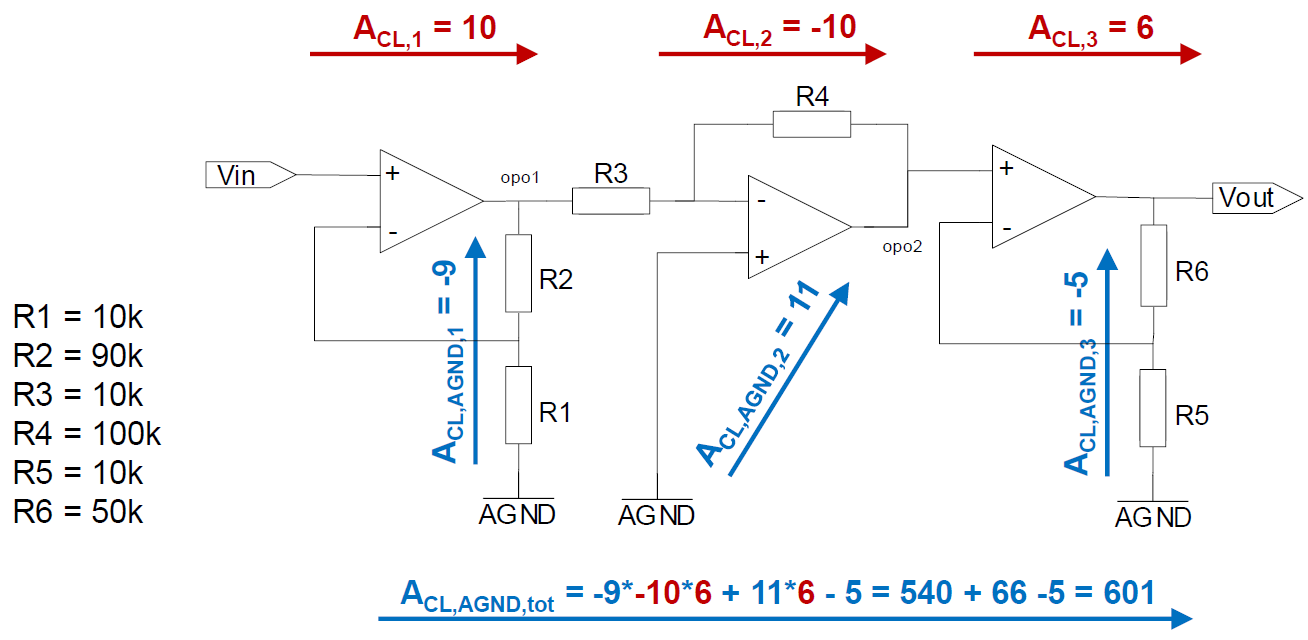
\includegraphics[width=0.85\columnwidth]{images/mehrstufige_verstaerker.png}
\end{center}


\subsection{Gesteuerte Quellen}

\subsubsection{Stromgesteuerte Stromquellen}

\begin{minipage}[c]{0.4\columnwidth}
	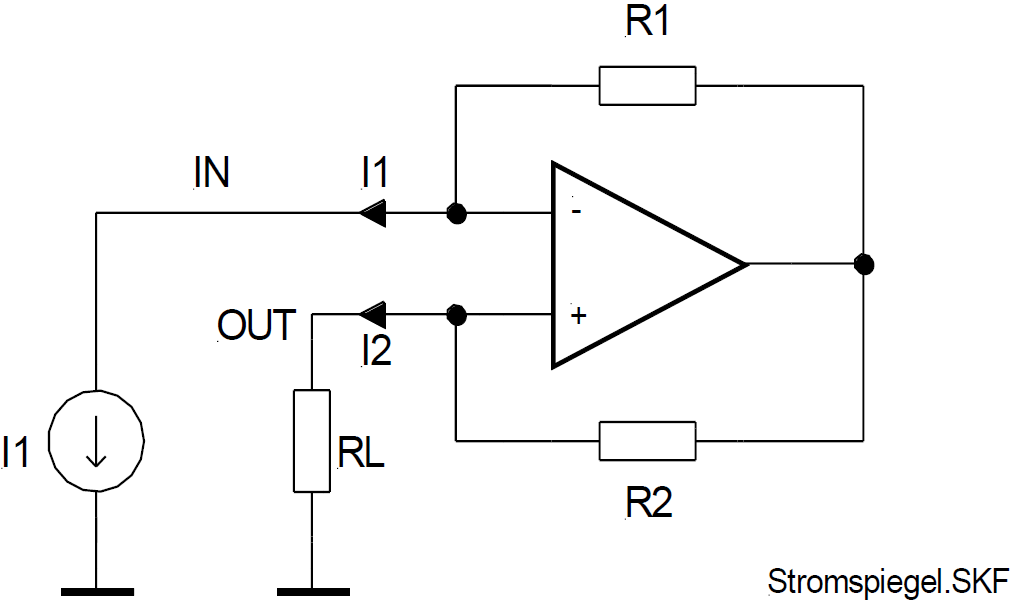
\includegraphics[width=\columnwidth]{images/stromspiegel_OPV.png}
\end{minipage}
\hfill
\begin{minipage}[c]{0.48\columnwidth}
	$$ V_{R1} = V_{R2} \qquad R_1 \, I_1 = R_2 \, I_2 $$
	$$ \boxed{ A_i = \frac{I_2}{I_1} = \frac{R_1}{R_2} }$$
\end{minipage}


\subsubsection{Spannungsgesteuerte Stromquellen}

\begin{minipage}[c]{0.4\columnwidth}
	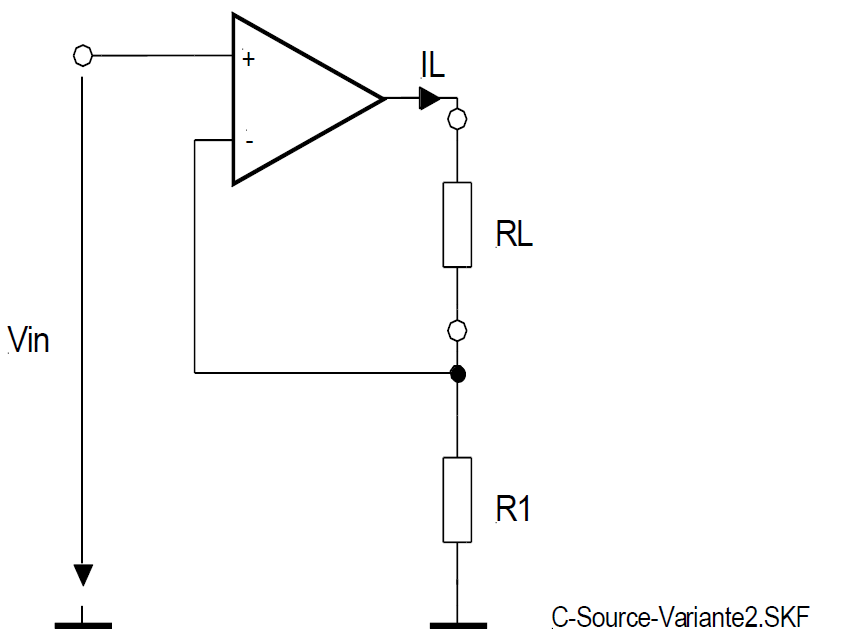
\includegraphics[width=\columnwidth]{images/spannungsgesteuerte_stromquelle_V1.png}
	$$ I_L = \frac{V_{\rm in}}{R_1}$$
	Nachteil: Last muss 'floating' sein
\end{minipage}
\hfill
\begin{minipage}[c]{0.48\columnwidth}
	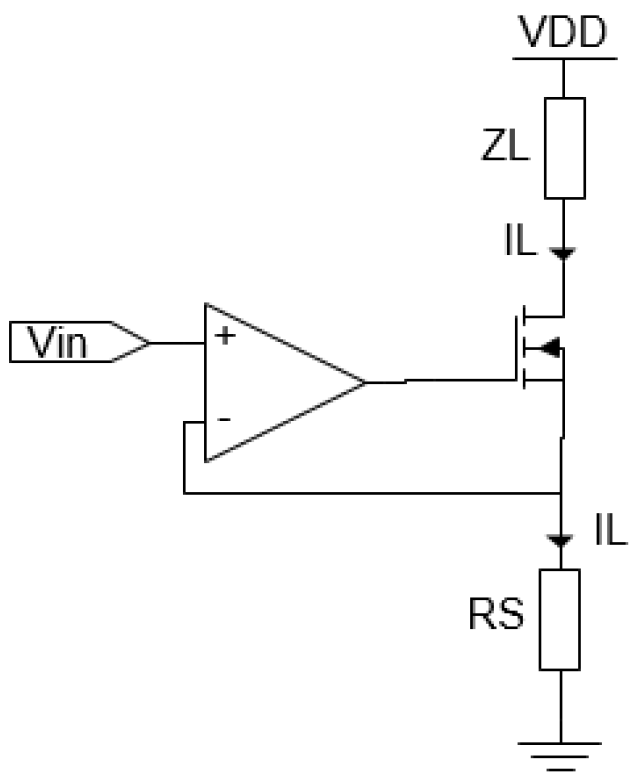
\includegraphics[width=0.6\columnwidth]{images/spannungsgesteuerte_stromquelle_V2.png}
	$$ I_L = \frac{V_{\rm in}}{R_s}$$
\end{minipage}


\subsection{Einfache Filterschaltungen mit OpAmps}

\subsubsection{Integratoren}

\begin{tabular}{ll}
	RL-Integrator:	& Spulen sind nichtideal und teuer 		\\
					& Spulen erzeugen oft Oszillationen 	\\
	RC-Integrator: 	& fast immer für aktive Filter verwendet
\end{tabular}

\vspace{0.2cm}

\begin{minipage}[c]{0.4\columnwidth}
	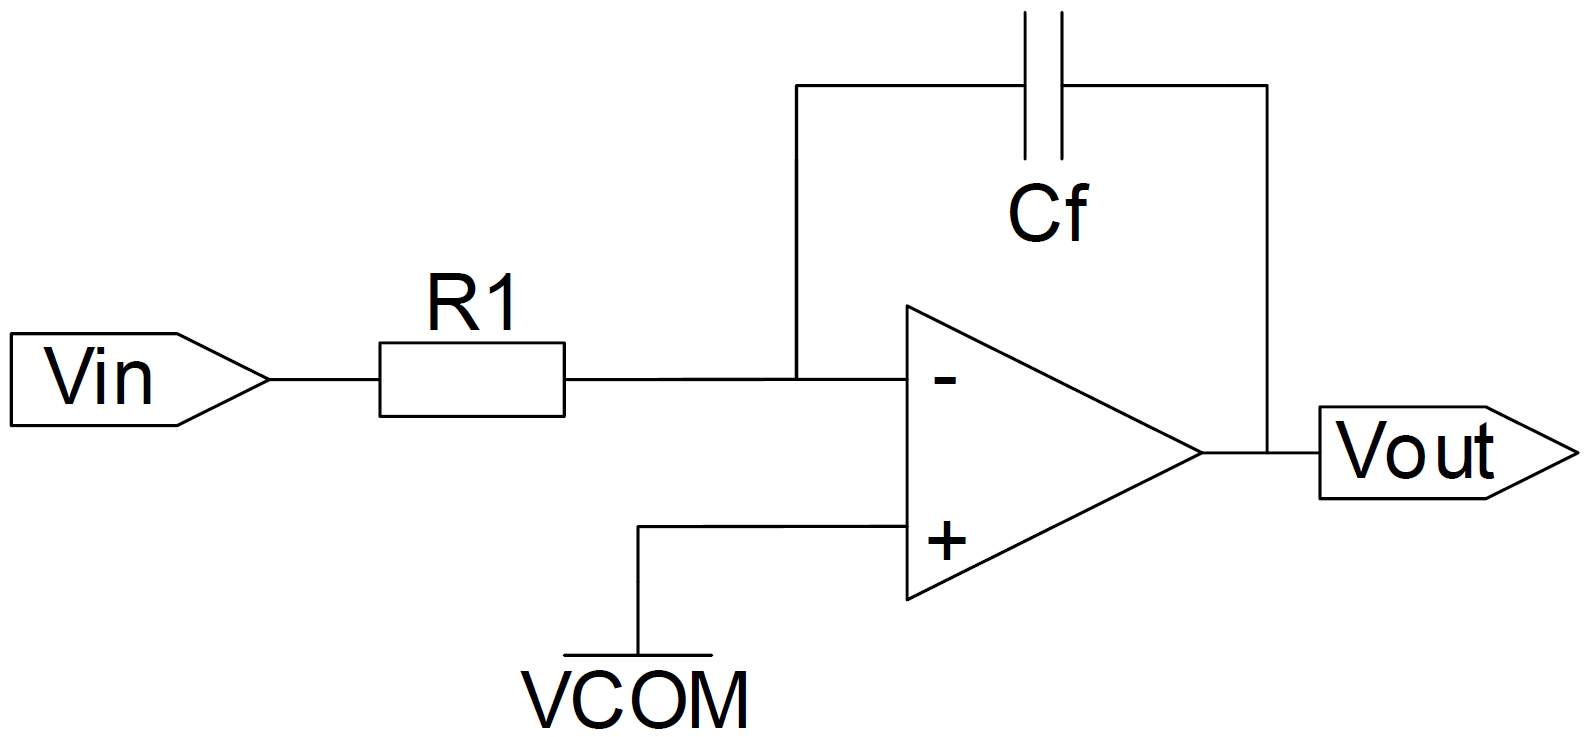
\includegraphics[width=\columnwidth]{images/integrator.png} 
\end{minipage}
\hfill
\begin{minipage}[c]{0.58\columnwidth}
	$$ \boxed{ V_{\rm out}(t) = - \frac{1}{R_1 \cdot C_f} \int\limits_0^t V_{\rm in}(\tau) \, \diff \tau + V_{C_f}(0) } $$
	$$ \boxed{ V_{\rm out}(t) = - \frac{1}{C_f} \int\limits_0^t I_{C_f}(\tau) \, \diff \tau + V_{C_f}(0) } $$
\end{minipage}


\subsubsection{Differenzierer}

\begin{minipage}[c]{0.4\columnwidth}
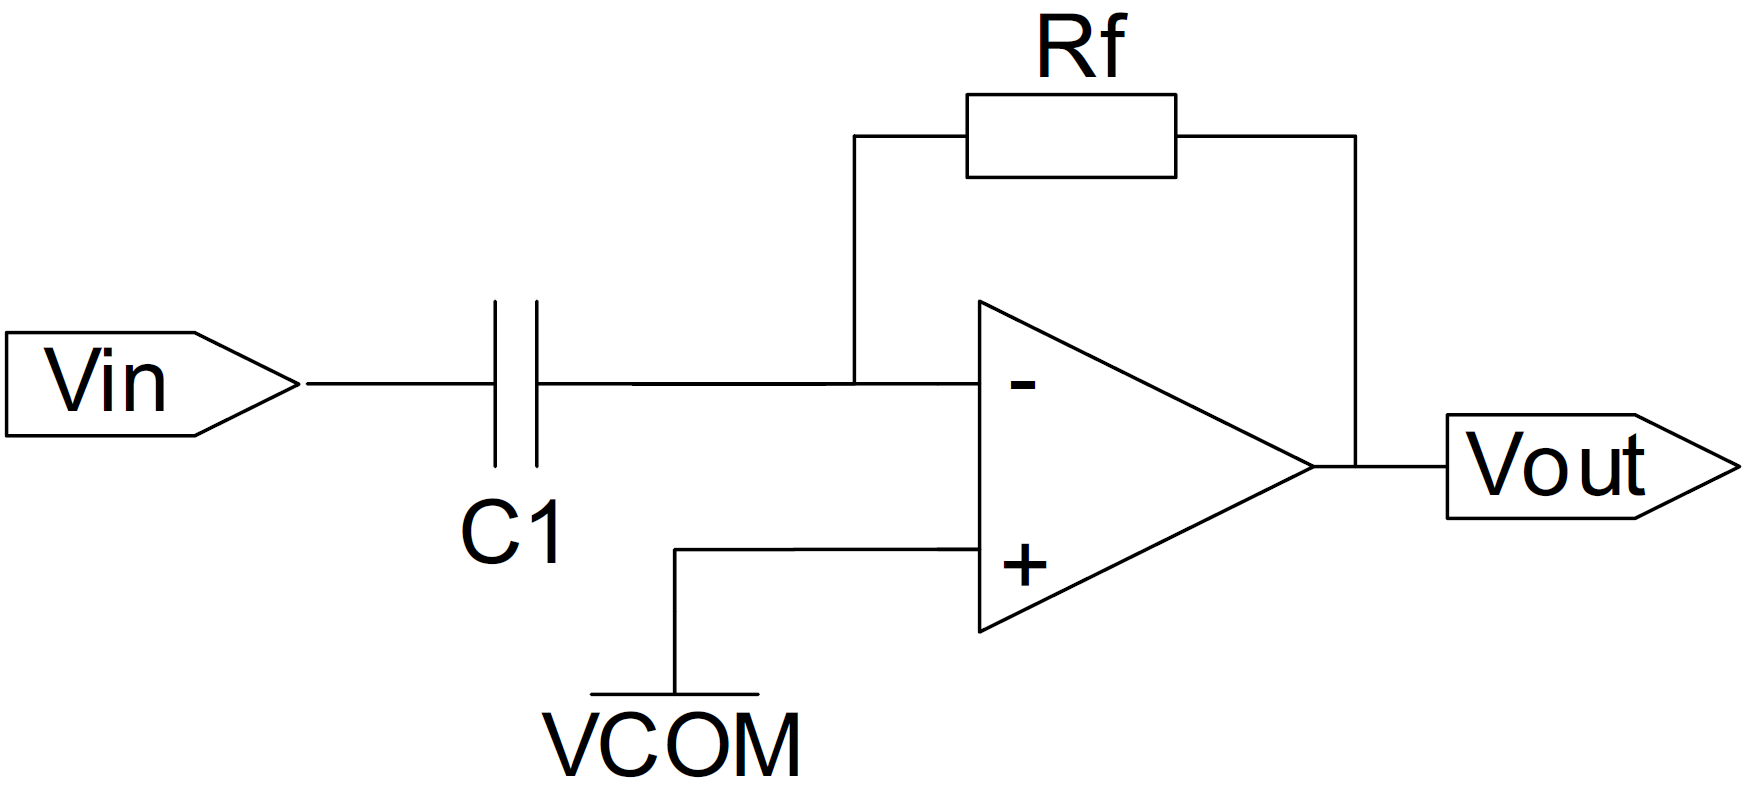
\includegraphics[width=\columnwidth]{images/differenzierer.png}
\end{minipage}
\hfill
\begin{minipage}[c]{0.58\columnwidth}
	$$ \boxed{ V_{\rm out} = - R_f \cdot C_1 \frac{\diff V_{\rm in}}{\diff t} } $$
	$$ \boxed{ i_{c} = C_1 \frac{\diff v_c}{\diff t} = C_1 \frac{\diff V_{\rm in}}{\diff t} } $$
\end{minipage}

\vspace{0.2cm}

\myul{\textbf{Differenzierer im Frequenzbereich}}

\vspace{0.1cm}

\begin{itemize}
	\item Hohe Freqeunzen werden mehr verstärkt
	\item Rückkopplungsfunktion ist Tiefpass
	\item Realer OpAmp bildet auch Tiefpass
	\item Beide Tiefpasse erzeugen zusammen $180 \, \degree$ Phasenschiebung \\
		\textrightarrow\ Mitkopplung \textrightarrow\ Schwingung 
	\item Kleines $C$ parallel zu $R_f$ unterdrückt Schwingungen
\end{itemize}


\subsubsection{Tiefpass}

\begin{minipage}[c]{0.4\columnwidth}
	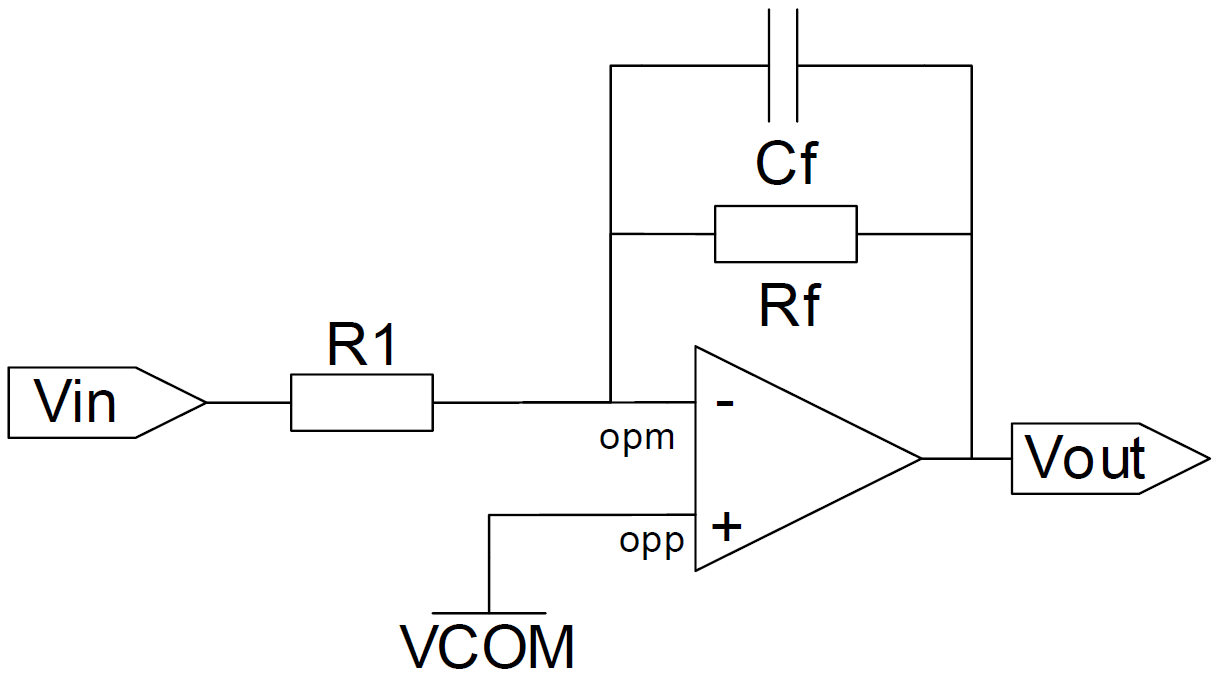
\includegraphics[width=\columnwidth]{images/tiefpass.png}
\end{minipage}
\hfill
\begin{minipage}[c]{0.58\columnwidth}
	\begin{tabular}{ll}
		\cbl{Tiefe $f$}:  	& $R_f$ limitiert Verstärkung 	\\
							& $I_{C_f} = 0$ (Unterbruch) 	\\
		\cgn{Hohe $f$}:		& $-20 \, \deci \bel$ / Dek
	\end{tabular}

	$$ \cbl{ \boxed{ V_{\rm out} = - \frac{R_f}{R_1} \cdot V_{\rm in} } } \qquad \cgn{ \boxed{ f_g = \frac{1}{2 \, \pi \cdot R_f \cdot C_1} } } $$
\end{minipage}


\subsubsection{Bandpass}

\begin{minipage}[c]{0.48\columnwidth}
	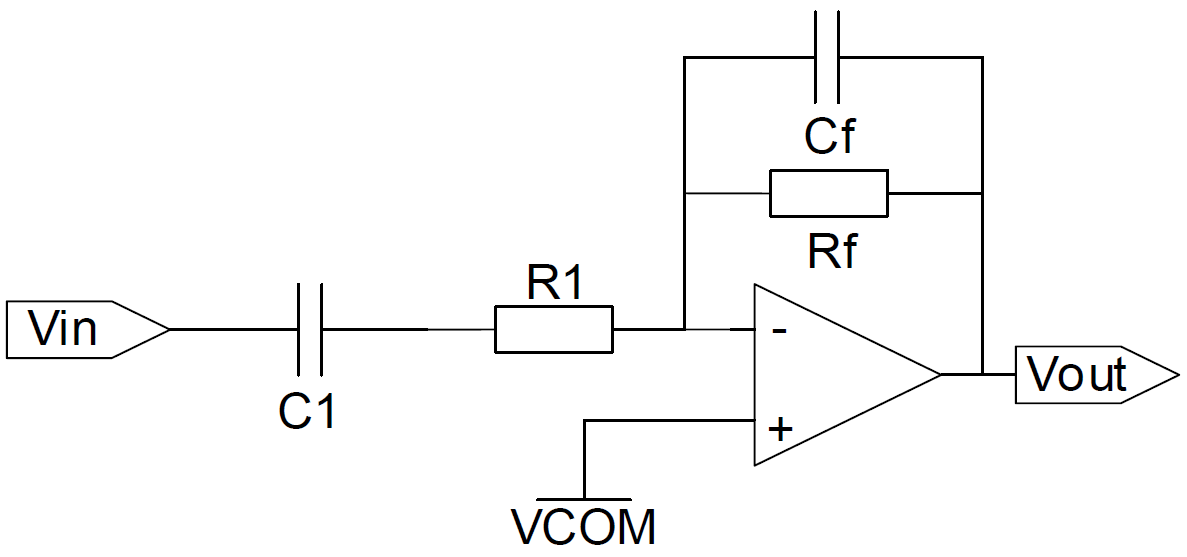
\includegraphics[width=\columnwidth]{images/bandpass.png} 
\end{minipage}
\hfill
\begin{minipage} [c]{0.48\columnwidth}
	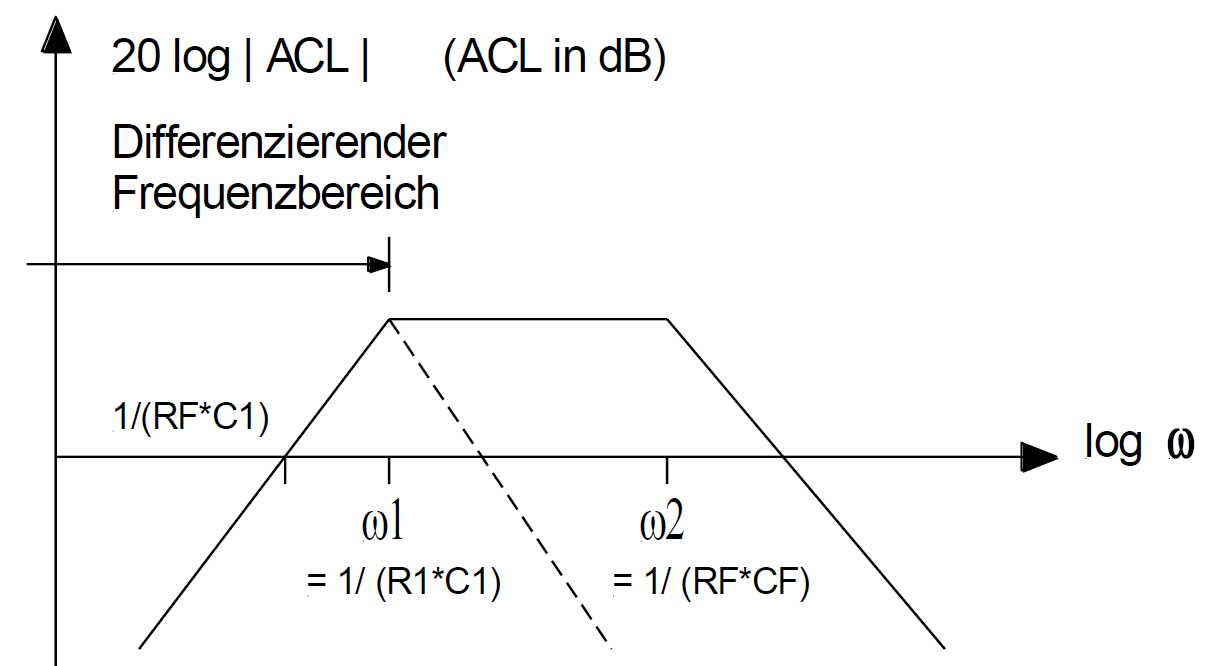
\includegraphics[width=\columnwidth]{images/bandpass_amplitudengang.png}
\end{minipage}

\vspace{0.2cm}

\begin{tabular}{ll}
	$R_1$ & limitiert Eingangsstrom 						\\
	$C_f$ & limitiert $V_{\rm out}$ bei hohen Frequenzen 
\end{tabular}


\subsubsection{Allpass}

\begin{itemize}
	\item Betrag der Verstärkung $= 1$ ($-1$ @ $180 \, \degree$ \textrightarrow\ $1$ @ $0 \, \degree$)
	\item Phase ändert mit der Frequenz von $180 \, \degree$ auf $0 \, \degree $
\end{itemize}

\vspace{0.2cm}

\begin{minipage}[c]{0.4\columnwidth}
	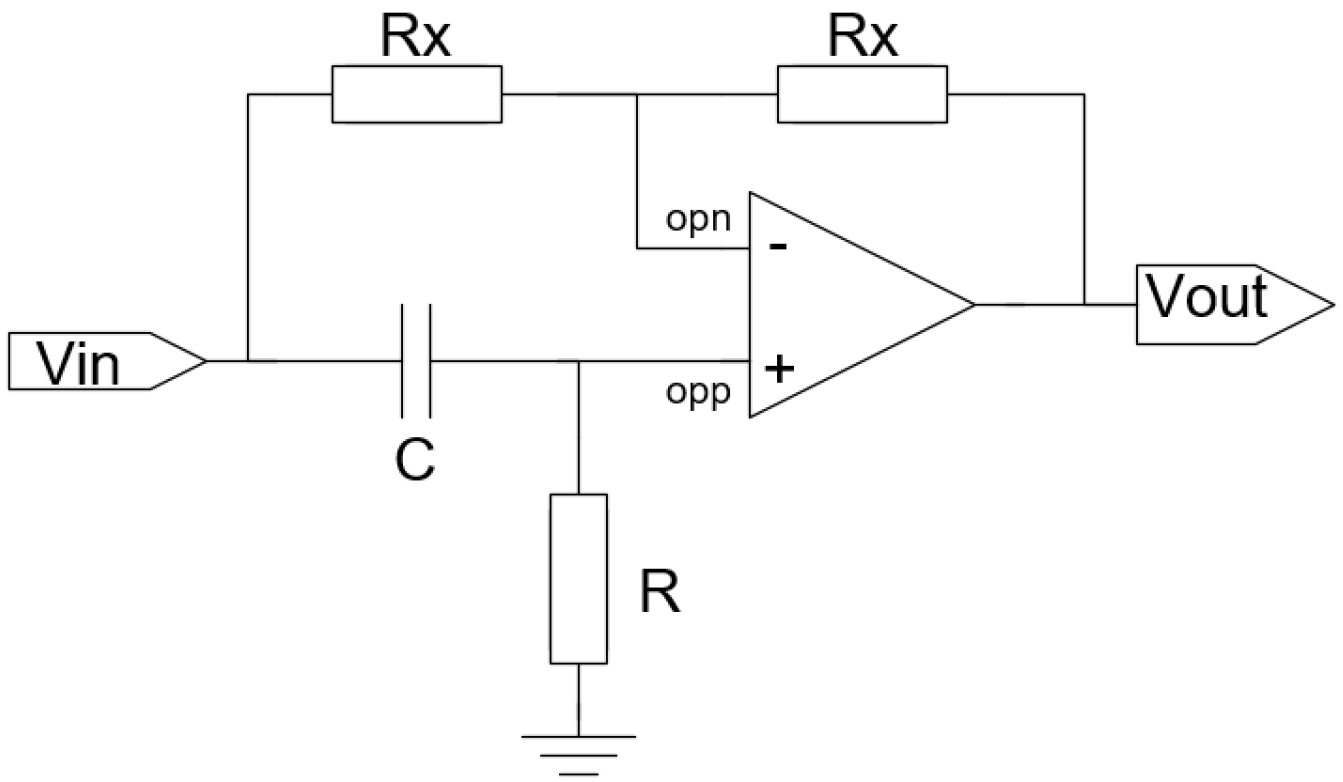
\includegraphics[width=\columnwidth]{images/allpass.png}
\end{minipage}
\hfill
\begin{minipage}[c]{0.58\columnwidth}
	\begin{tabular}{ll}
		\cbl{tiefe $f$}:	& $C$ sperrt (Unterbruch) 										\\
							& \textrightarrow\ $I_{C_f} = 0$  								\\
		\cgn{hohe $f$}: 	& $C$ ist Kurzschluss 											\\
							& $V_{\rm opn} = V_{\rm opp}$ \textrightarrow\ $I_{R_x} = 0$ 
	\end{tabular}

	$$ \cbl{ \boxed{ V_{\rm out} = - \frac{R_x}{R_x} \cdot V_{\rm in} = - V_{\rm in} } } \qquad 
	   \cgn{ \boxed{ V_{\rm out} = V_{\rm in} } } $$
\end{minipage}


\subsection{Nichtidealitäten von OpAmps}

\begin{tabular}{ll}
	\tabitem Endliche Verstärkung:	& $V_d = V_{\rm opp} - V_{\rm opn} = \frac{V_{\rm out}}{A_{\rm ol}}$	\\
	\tabitem Offset-Spannung:		& $V_{\rm os}$: Gleich verstärkt wie $V_{\rm opp}$
\end{tabular}


\subsubsection{Eingangsstromfehler - Bias-Strom $\rm{I_B}$}

\begin{minipage}[c]{0.48\columnwidth}
	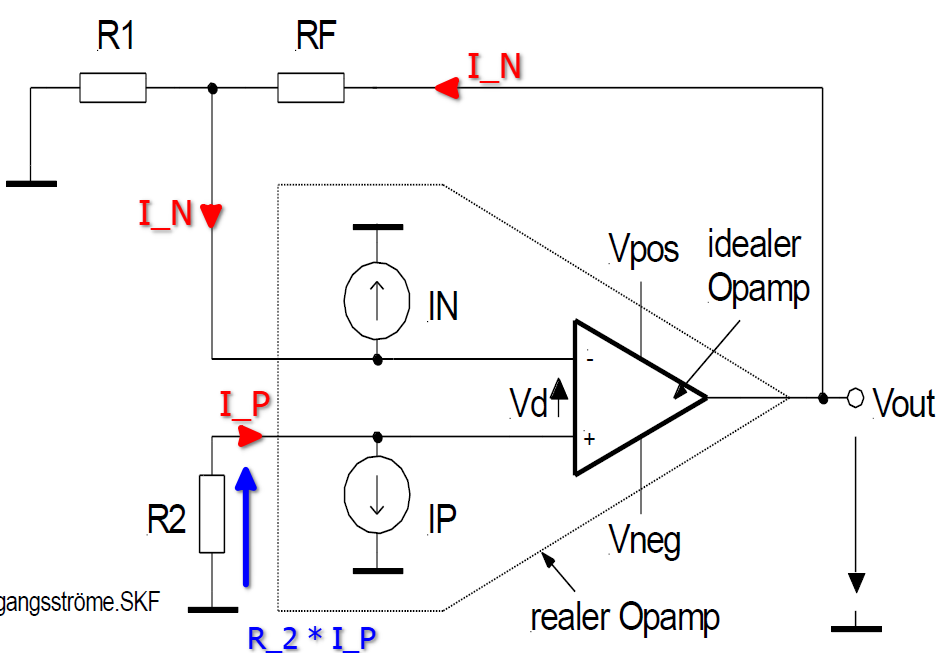
\includegraphics[width=\columnwidth]{images/bias-strom_grafik.png} 
\end{minipage}
\hfill
\begin{minipage}[c]{0.48\columnwidth}
	Modellierung durch Stromquellen \\
	$I_P$, $I_N$  

	\vspace{0.2cm}

	$V_{\rm outE} =$ Fehlerspannung aufgrund von $I_B, \, I_N$

	$$ I_B = \frac{I_P + I_N}{2} $$
\end{minipage}

\vspace{0.2cm}
$$ \boxed{ V_{\rm outE} = V_{\rm outE(N)} +  V_{\rm outE(P)} = I_N \, R_F - R_2 \, I_P \Bigg( \frac{R_F + R_1}{R_1}  \Bigg) } $$

$$ \text{Kompensation:} \quad I_B = \frac{I_P + I_N}{2}: \quad  V_{\rm outE} \overset{!}{=} 0 $$ 
$$ I_N = I_P: \quad R_F = R_2 \, \Bigg( \frac{R_F + R_1}{R_1} \Bigg) \quad \boxed{ R_2 = \frac{R_F \cdot R_1}{R_F + R_1} = R_F || R_1 } $$

\vspace{0.1cm}

\myul{\textbf{Bias-Strom-Kompensation mittels $\bm{R_2}$}}

\vspace{0.1cm}

\begin{minipage}[b]{0.3\columnwidth}
	\begin{center}
		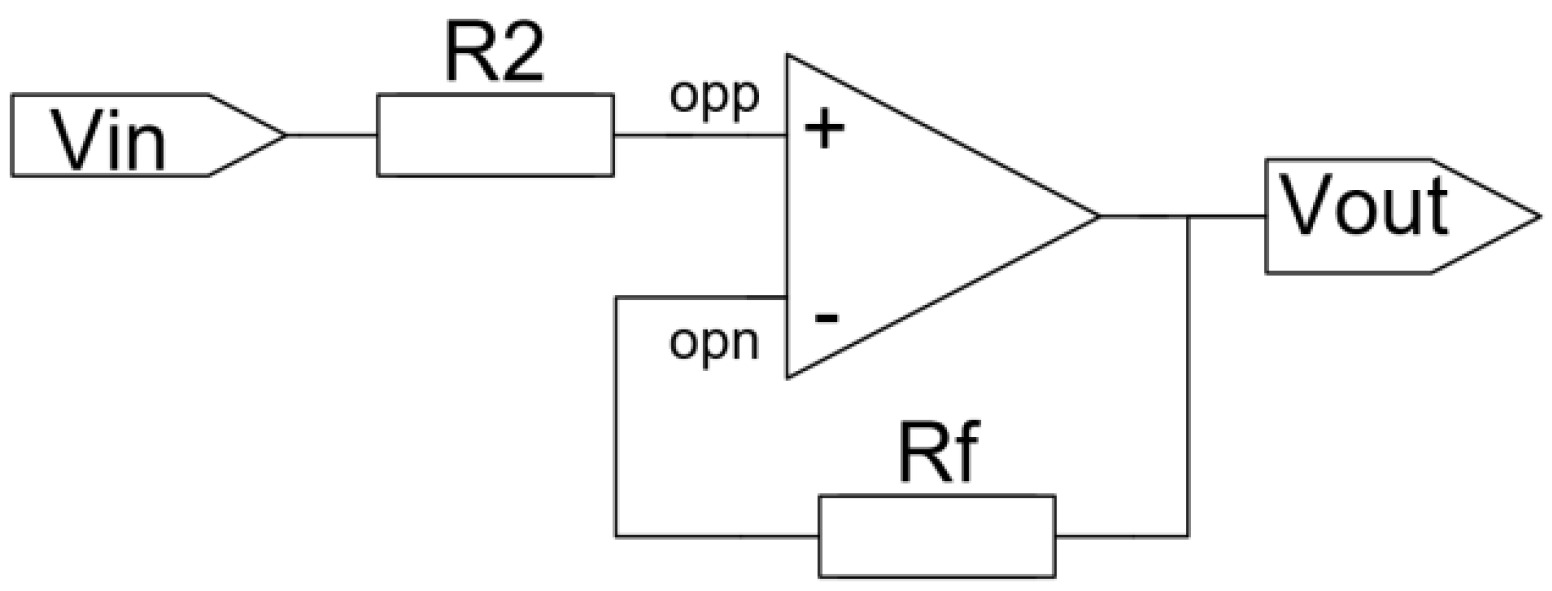
\includegraphics[width=\columnwidth]{images/kompensation_bias-strom_1.png}
		$$ R_2 = R_F $$
	\end{center}
\end{minipage}
\hfill
\begin{minipage}[b]{0.3\columnwidth}
	\begin{center}
		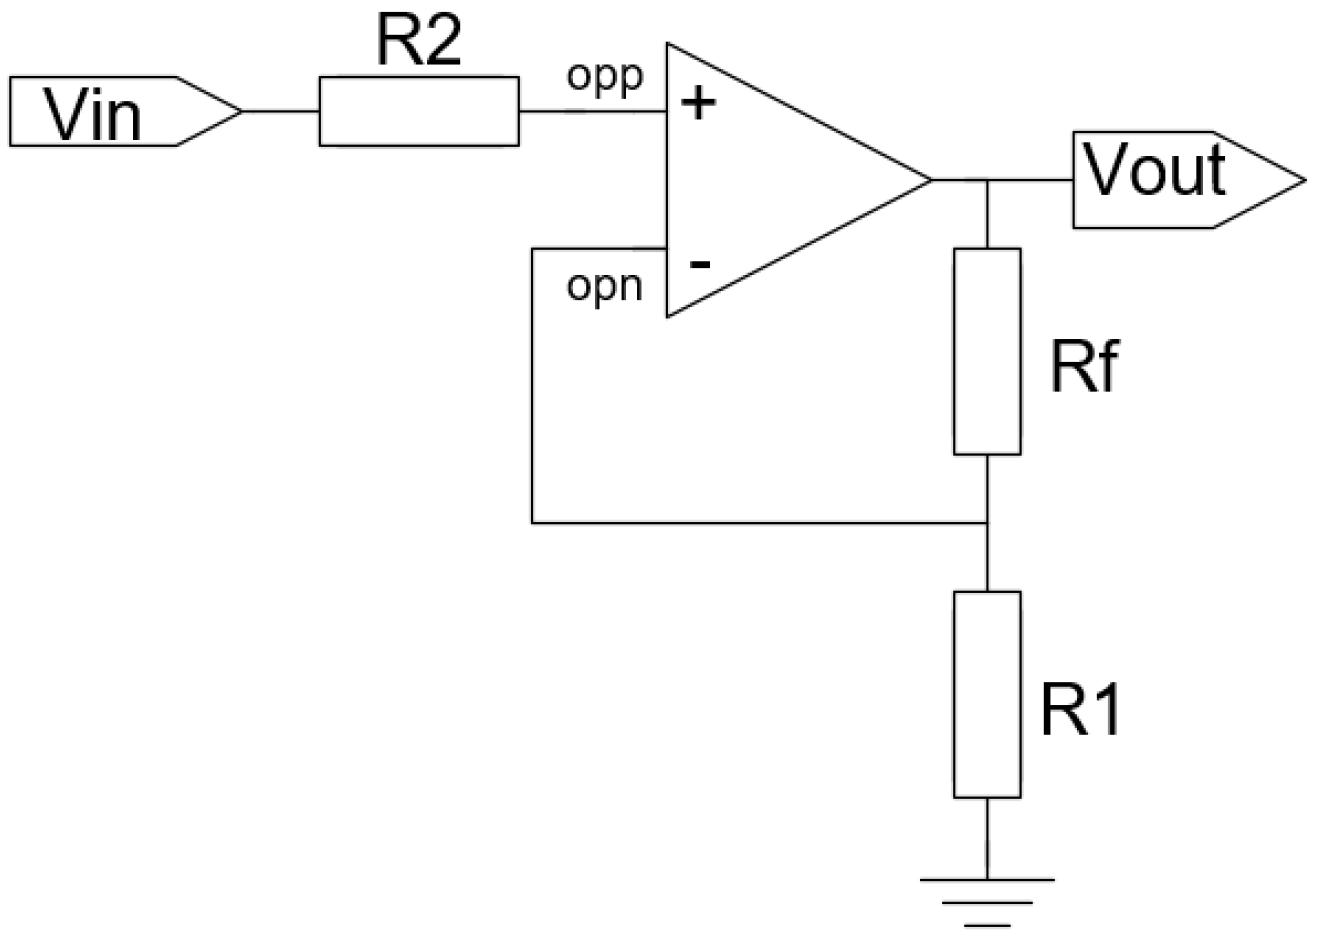
\includegraphics[width=\columnwidth]{images/kompensation_bias-strom_2.png}
		$$ R_2 = R_F || R_1 $$
	\end{center}
\end{minipage}
\hfill
\begin{minipage}[b]{0.3\columnwidth}
	\begin{center}
		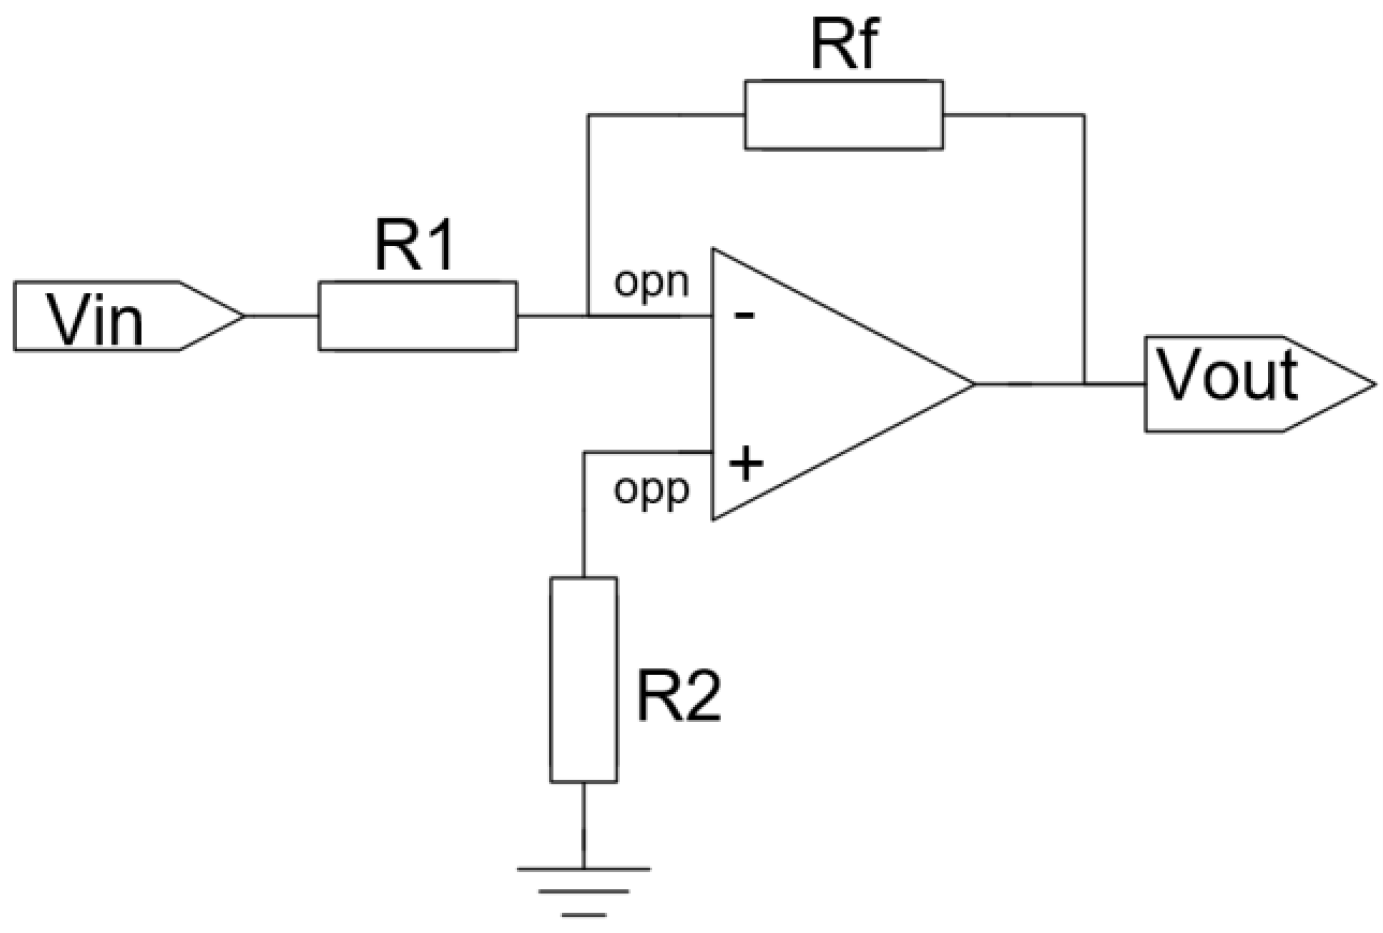
\includegraphics[width=\columnwidth]{images/kompensation_bias-strom_3.png}
		$$ R_2 = R_F || R_1 $$
	\end{center}
\end{minipage}


\subsubsection{Eingangsstromfehler - Offset-Strom $\bm{I_{\rm OS}}$}

Der Offset-Strom entsteht aufgrund von \textbf{Herstellungstoleranzen} und ist \textbf{nicht kompensierbar} 
$$ \text{Offset-Strom:} \quad I_{\rm OS} = I_P - I_N  $$

Wenn der Bias-Strom $I_B$ mittels $R_2$ kompensiert ist gilt: 

$$ \boxed{  V_{\rm outE} = R_F \cdot (I_N - I_P) = R_F \cdot I_{\rm OS} } $$

\textbf{ \textrightarrow\ Je kleiner $ \bm{R_F}$, desto kleiner die Fehlerspannung!}


\subsection{Dynamisches Verhalten von OpAmps}

\subsubsection{Verstärkungs-Bandbreite-Produkt (GB(W)P)}

\begin{minipage}[c]{0.45\columnwidth}
	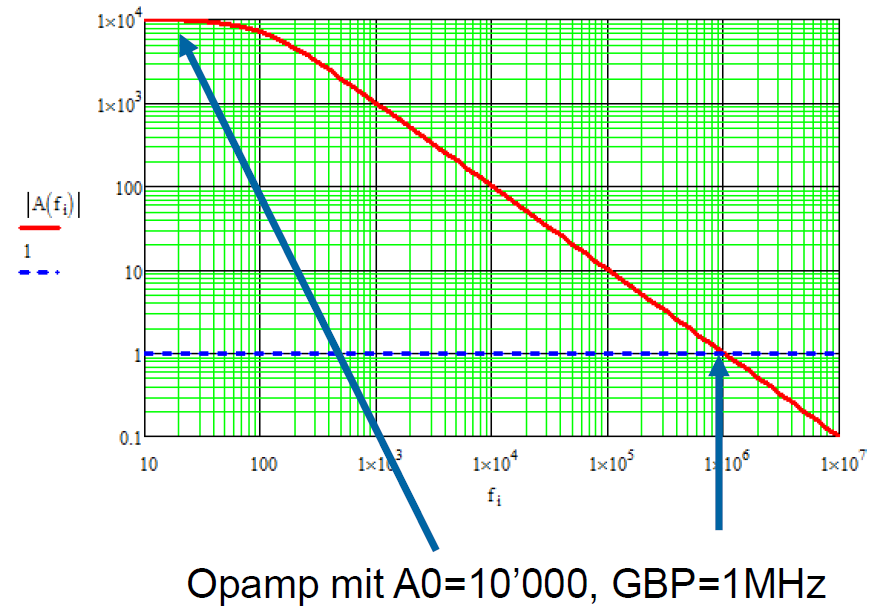
\includegraphics[width=\columnwidth]{images/verstaerkungs-bandbreite-produkt.png} 
\end{minipage}
\hfill
\begin{minipage}[c]{0.48\columnwidth}
	Verstärkung des OpAmps sinkt mit höherer Frequenz \\
	Datenblatt anstelle von $A_{\rm ol}$ (da Frequnzabhängig)

	$$ \boxed{ A_{\rm cl} \cdot f_{3 \deci \bel} = \mathrm{GBWP} = \const } $$
\end{minipage}


\subsubsection{Common Mode Rejection Ratio (CMRR)}

\begin{minipage}[c]{0.48\columnwidth}
	$$ \boxed{ \mathrm{CMRR} = \frac{\diff V_{\rm CM}}{\diff V_{\rm os}} }$$
\end{minipage}
\hfill
\begin{minipage}[c]{0.48\columnwidth}
	$$ \boxed{ V_{\rm CM} = \frac{V_{\rm opp} + V_{\rm opn}}{2} } $$
\end{minipage}


\subsubsection{Power Supply Noise Rejection Ratio (PSNRR)}

$$ \boxed{ \mathrm{PSNRR} = \frac{\diff V_{\rm supply}}{\diff V_{\rm os}} } $$


\subsection{Anstiegszeit (Slew-Rate)}

\begin{minipage}[c]{0.48\columnwidth}
	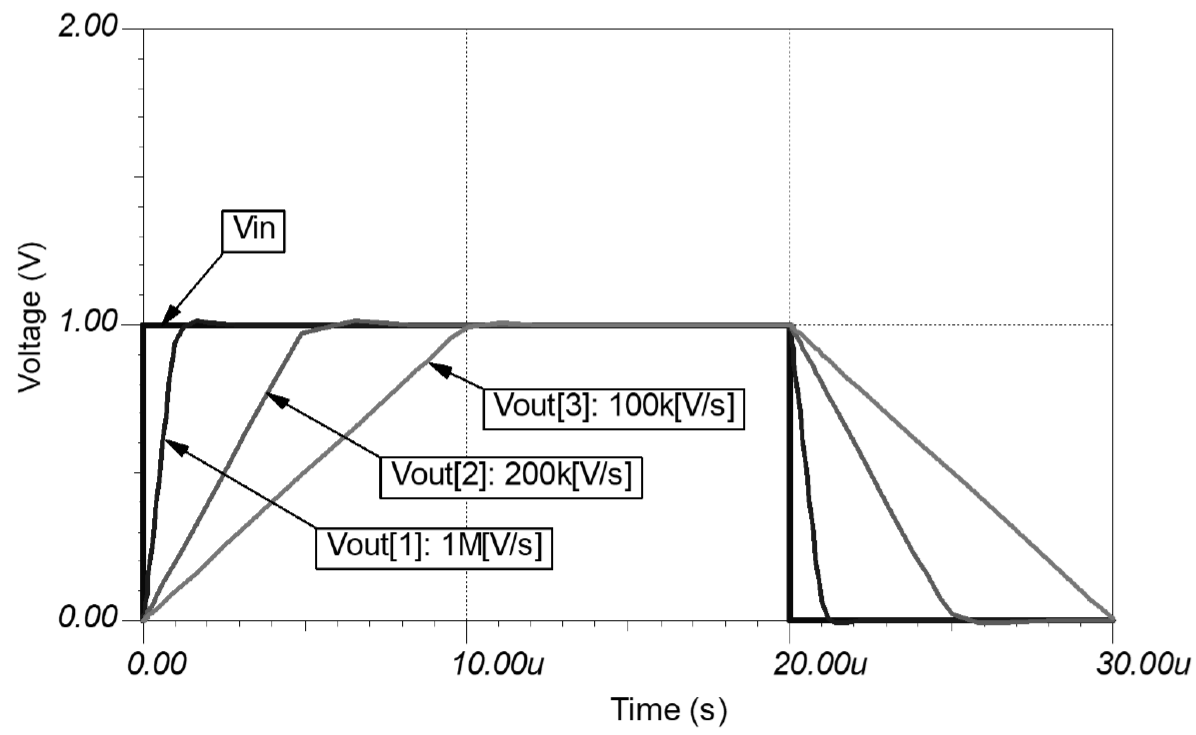
\includegraphics[width=\columnwidth]{images/slew_rate.png} 
\end{minipage}
\hfill
\begin{minipage}[c]{0.48\columnwidth}
	\raggedright
	Maximal mögliche Änderungsgeschwindigkeit der Ausgangsspannung des OpAmps

	$$ \boxed{ \mathrm{SR} = \Bigl| \frac{\diff V_{\rm out}}{\diff t} \Bigr|_{\rm max} } $$
\end{minipage}

Wenn der Ausgang schneller ändern soll als die Slew-Rate 'erlaubt', so wird das Ausgangssignal \textbf{begrenzt bzw. verformt} \\
\textrightarrow\ Signal verformt / Amplitude reduziert \textrightarrow\ Dreieck statt Sinus 